% !TEX encoding = UTF-8 Unicode
% !TEX TS-program = XeLaTeX
% !TEX root = ParliamentUserGuide.tex

%%%%%%%%%%%%%%%%%%%%%%%%%%%%%%%%%%%%%%%%%%%%%%%%%%
\chapter{Introduction}

\pmnt{} is a high-performance triple store and reasoner designed for the Semantic Web\urlcite{http://www.w3.org/2001/sw/}.  Parliament was originally developed under the name DAML DB\urlcite{http://www.daml.org/2001/09/damldb/} and was extended by Raytheon BBN Technologies (hereafter referred to simply as ``BBN'') for internal use in its R\&D programs.  BBN released Parliament as an open source project under the BSD license\urlcite{http://opensource.org/licenses/bsd-license.php} on SemWebCentral\urlcite{http://parliament.semwebcentral.org/} in 2009.

\pmnt{} is a trademark of Raytheon BBN Technologies, Inc., and is so-named because a group of owls is properly called a \emph{parliament} of owls.

%%%%%%%%%%%%%%%%%%%%%%%%%%%%%%%%%%%%%%%%%%%%%%%%%%
\section{Background}

The Semantic Web employs a different data model than a relational database.  A relational database stores data in tables (rows and columns) while RDF\urlcite{http://www.w3.org/RDF/} represents data as a directed graph of ordered triples of the form (subject, predicate, object).  Accordingly, a Semantic Web data store is often called a graph store, knowledge base, or triple store.

A relational database can store a directed graph, and some graph stores are in fact implemented as a thin interface layer wrapping a relational database.  However, the query performance of such implementations is usually poor.  This is because the only straightforward way to store the graph with the required level of generality is to use a single table to store all the triples, and this schema tends to defeat relational query optimizers.

Early in the Semantic Web's evolution, BBN encountered exactly this problem, and so the graph store we now call \emph{Parliament} was born.  The goal of Parliament was to create a storage mechanism optimized specifically to the needs of the Semantic Web, and the result was a dramatic speed boost for BBN's Semantic Web programs.  Since its initial conception, Parliament has served as a core component of several projects at BBN for a number of U.S.\ Government customers.

%%%%%%%%%%%%%%%%%%%%%%%%%%%%%%%%%%%%%%%%%%%%%%%%%%
\section{\protect\pmnt{} Architecture}

Parliament combines customized versions of the Web interface and query processor of Jena\urlcite{https://jena.apache.org/} with a high-performance storage engine and an innovative storage layout to deliver a complete triple store solution that is compatible with W3C's RDF, OWL\urlcite{http://www.w3.org/2007/OWL/}, and SPARQL\urlcite{http://www.w3.org/2009/sparql/wiki/Main\_Page} standards.

In addition, Parliament includes a high-performance rule engine, which applies a set of inference rules to the directed graph of data in order to derive new facts.  This enables Parliament to automatically and transparently infer additional facts and relationships in the data to enrich query results.  Parliament's rule engine currently implements all of RDFS inference plus selected elements of OWL RL.

Figure~\ref{figure-parliament-layers} depicts the layered architecture of Parliament.  The storage layer of Parliament is written in C++, while the remainder is Java code.  Integrated with the Jena query processor are a number of useful extras, such as support for named graphs, accelerated reification support, and temporal, geospatial, and numerical indexes.

\begin{figure}[htbp]
	\centering
	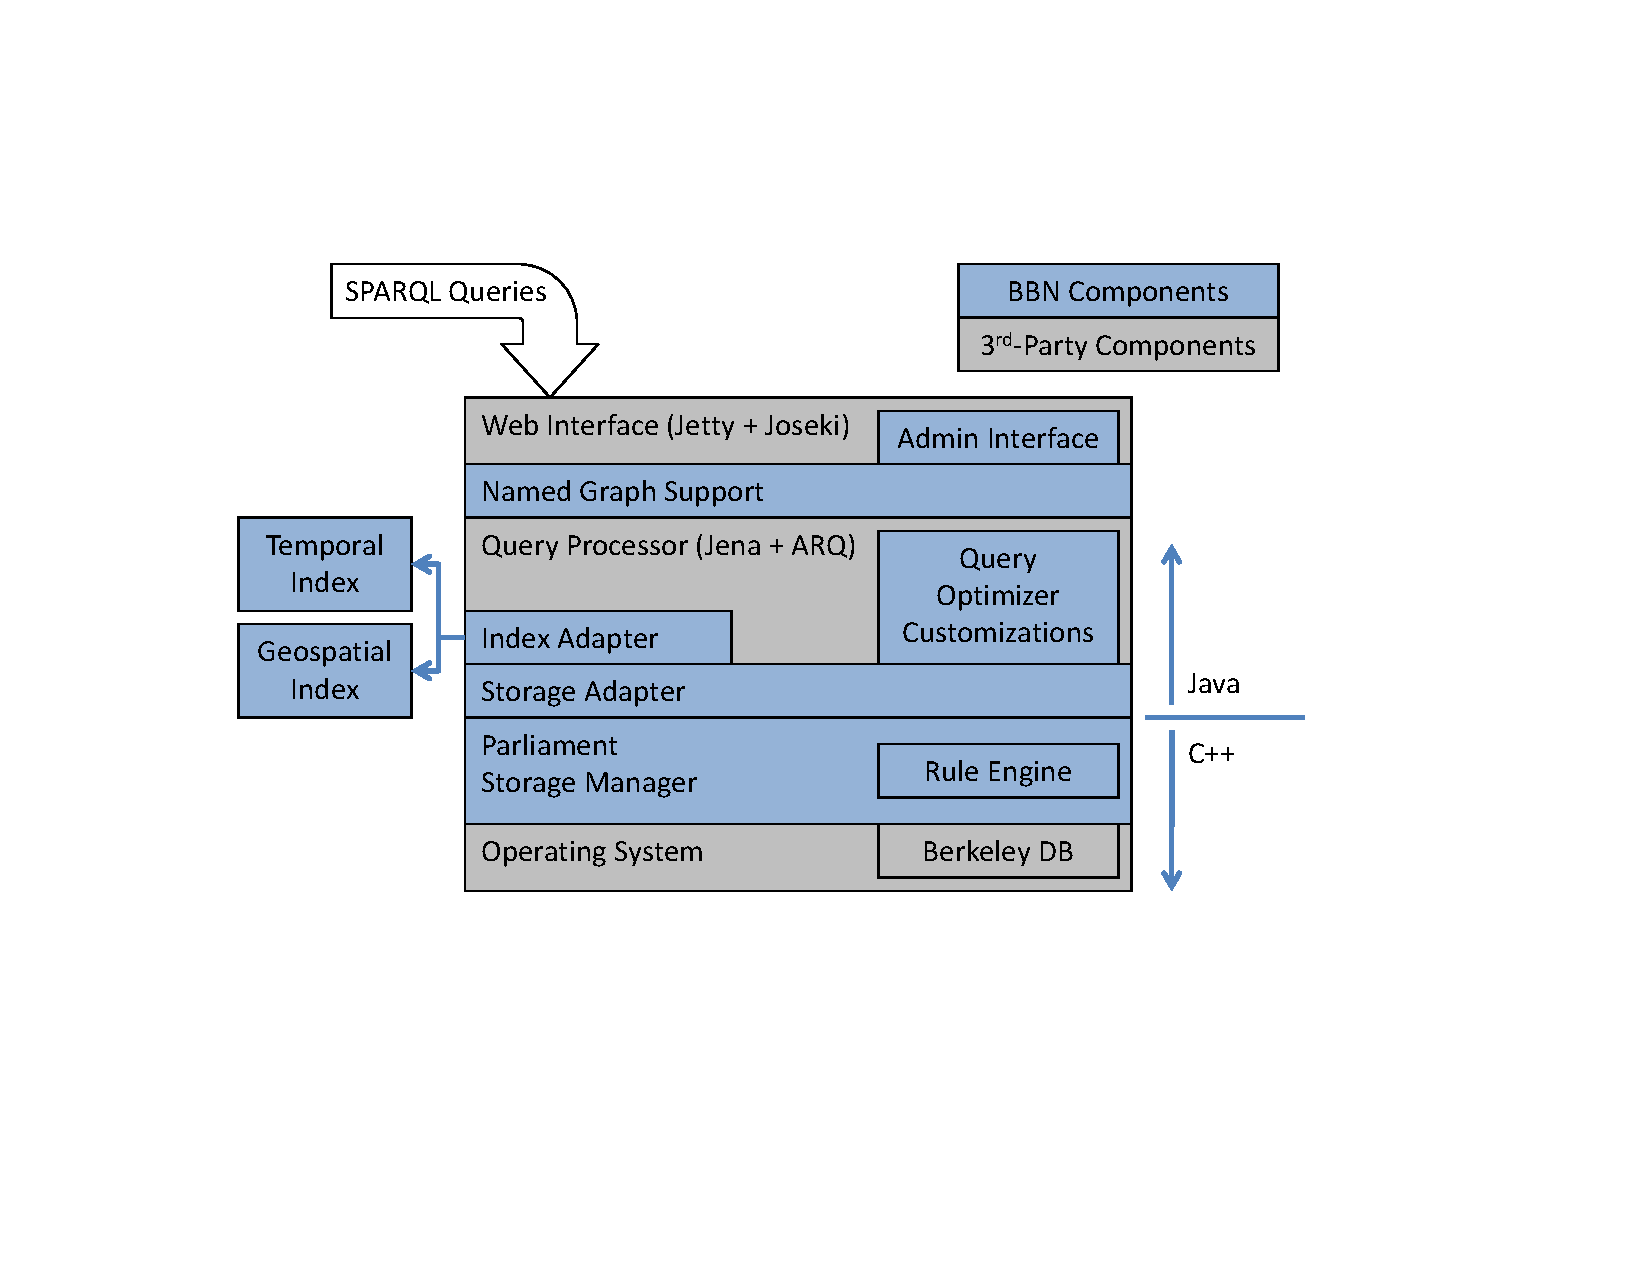
\includegraphics[width=1.0\textwidth]{architecture.pdf}
	\caption{Layered \protect\pmnt{} Architecture}
	\label{figure-parliament-layers}
\end{figure}
